\section{Error Analysis}

\subsection{Floating-Point Arithmetic and Roundoff Errors}

\begin{exercise}

	Calculate the following sum

	\[
		\sum_{n=1}^\infty {1\over n^2}={\pi^2\over 6}
		=\lim_{N\to\infty} S(N)
		\quad
		\text{with}
		\quad
		S(N)=\sum_{n=1}^N {1\over n^2}
	\]

	\begin{itemize}
		\item Calculate the sum in single precision using normal ordering,
		      $n=1,2,3,\ldots,N$.
		\item Calculate the sum in single precision using reverse ordering,
		      $n=N,\ldots,2,1$.
		\item Study the convergence of both implementations as a function of $N$
		      by plotting $|S(N)-\pi^2/6|$.
		\item Repeat (a)-(c) using double precision.
		\item Can you explain what happens?
	\end{itemize}

\end{exercise}

\begin{solution}
	The numerical evaluation of the infinite series $S(N)$ is performed by
	truncating the sum at a finite upper bound $N$. To investigate the impact of
	floating-point arithmetic and accumulation of round-off errors, the sum is
	implemented using both single precision (\texttt{Float32}) and double precision
	(\texttt{Float64}). For each precision type, two iterative strategies are
	employed:
	\begin{enumerate}
		\item \textbf{Normal ordering (Forward):} The loop iterates from $1$ to $N$,
		      adding successively smaller terms $\mathcal{O}(1/N^2)$ to an $\mathcal{O}(1)$
		      accumulator.
		\item \textbf{Reverse ordering (Backward):} The loop iterates from $N$ down
		      to $1$, aggregating the smallest terms first before adding them to the larger
		      components of the sum.
	\end{enumerate}
	The absolute error is evaluated against the analytical limit, $\pi^2/6$, with
	the error function defined as $\epsilon(N) = |S(N) - \pi^2/6|$.

	\paragraph{Results}
	The convergence of the sums was tested for $N$ ranging from $100$ to $10^6$.
	Table~\ref{tab:sum_errors} details the absolute numerical errors observed at $N
		= 999 \, 100$ for both precision types and summation orderings.

	\begin{center}
		\centering
		\captionof{table}{Absolute error of the numerical sum $S(N)$ evaluated at $N
				= 999 \, 100$ compared to the analytical value $\pi^2/6$.}
		\label{tab:sum_errors}
		\renewcommand{\arraystretch}{1.2}
		\begin{tabular}{@{}llc@{}}
			\toprule
			\textbf{Precision}        & \textbf{Ordering} & \textbf{Absolute Error} \\
			\midrule
			Single (\texttt{Float32}) & Normal            & $2.087 \times 10^{-4}$  \\
			                          & Reverse           & $1.073 \times 10^{-6}$  \\
			Double (\texttt{Float64}) & Normal            & $1.001 \times 10^{-6}$  \\
			                          & Reverse           & $1.001 \times 10^{-6}$  \\
			\bottomrule
		\end{tabular}
	\end{center}

	As expected, the theoretical truncation error of the series scales as
	$\mathcal{O}(1/N)$. A log-log plot (see Figure~\ref{fig:convergence}) visualizes
	the convergence behavior $\epsilon(N)$ as a function of $N$, illustrating
	significant deviations from the expected $\mathcal{O}(1/N)$ decay when using the
	normal ordering in single precision.

	\begin{center}
		\centering
		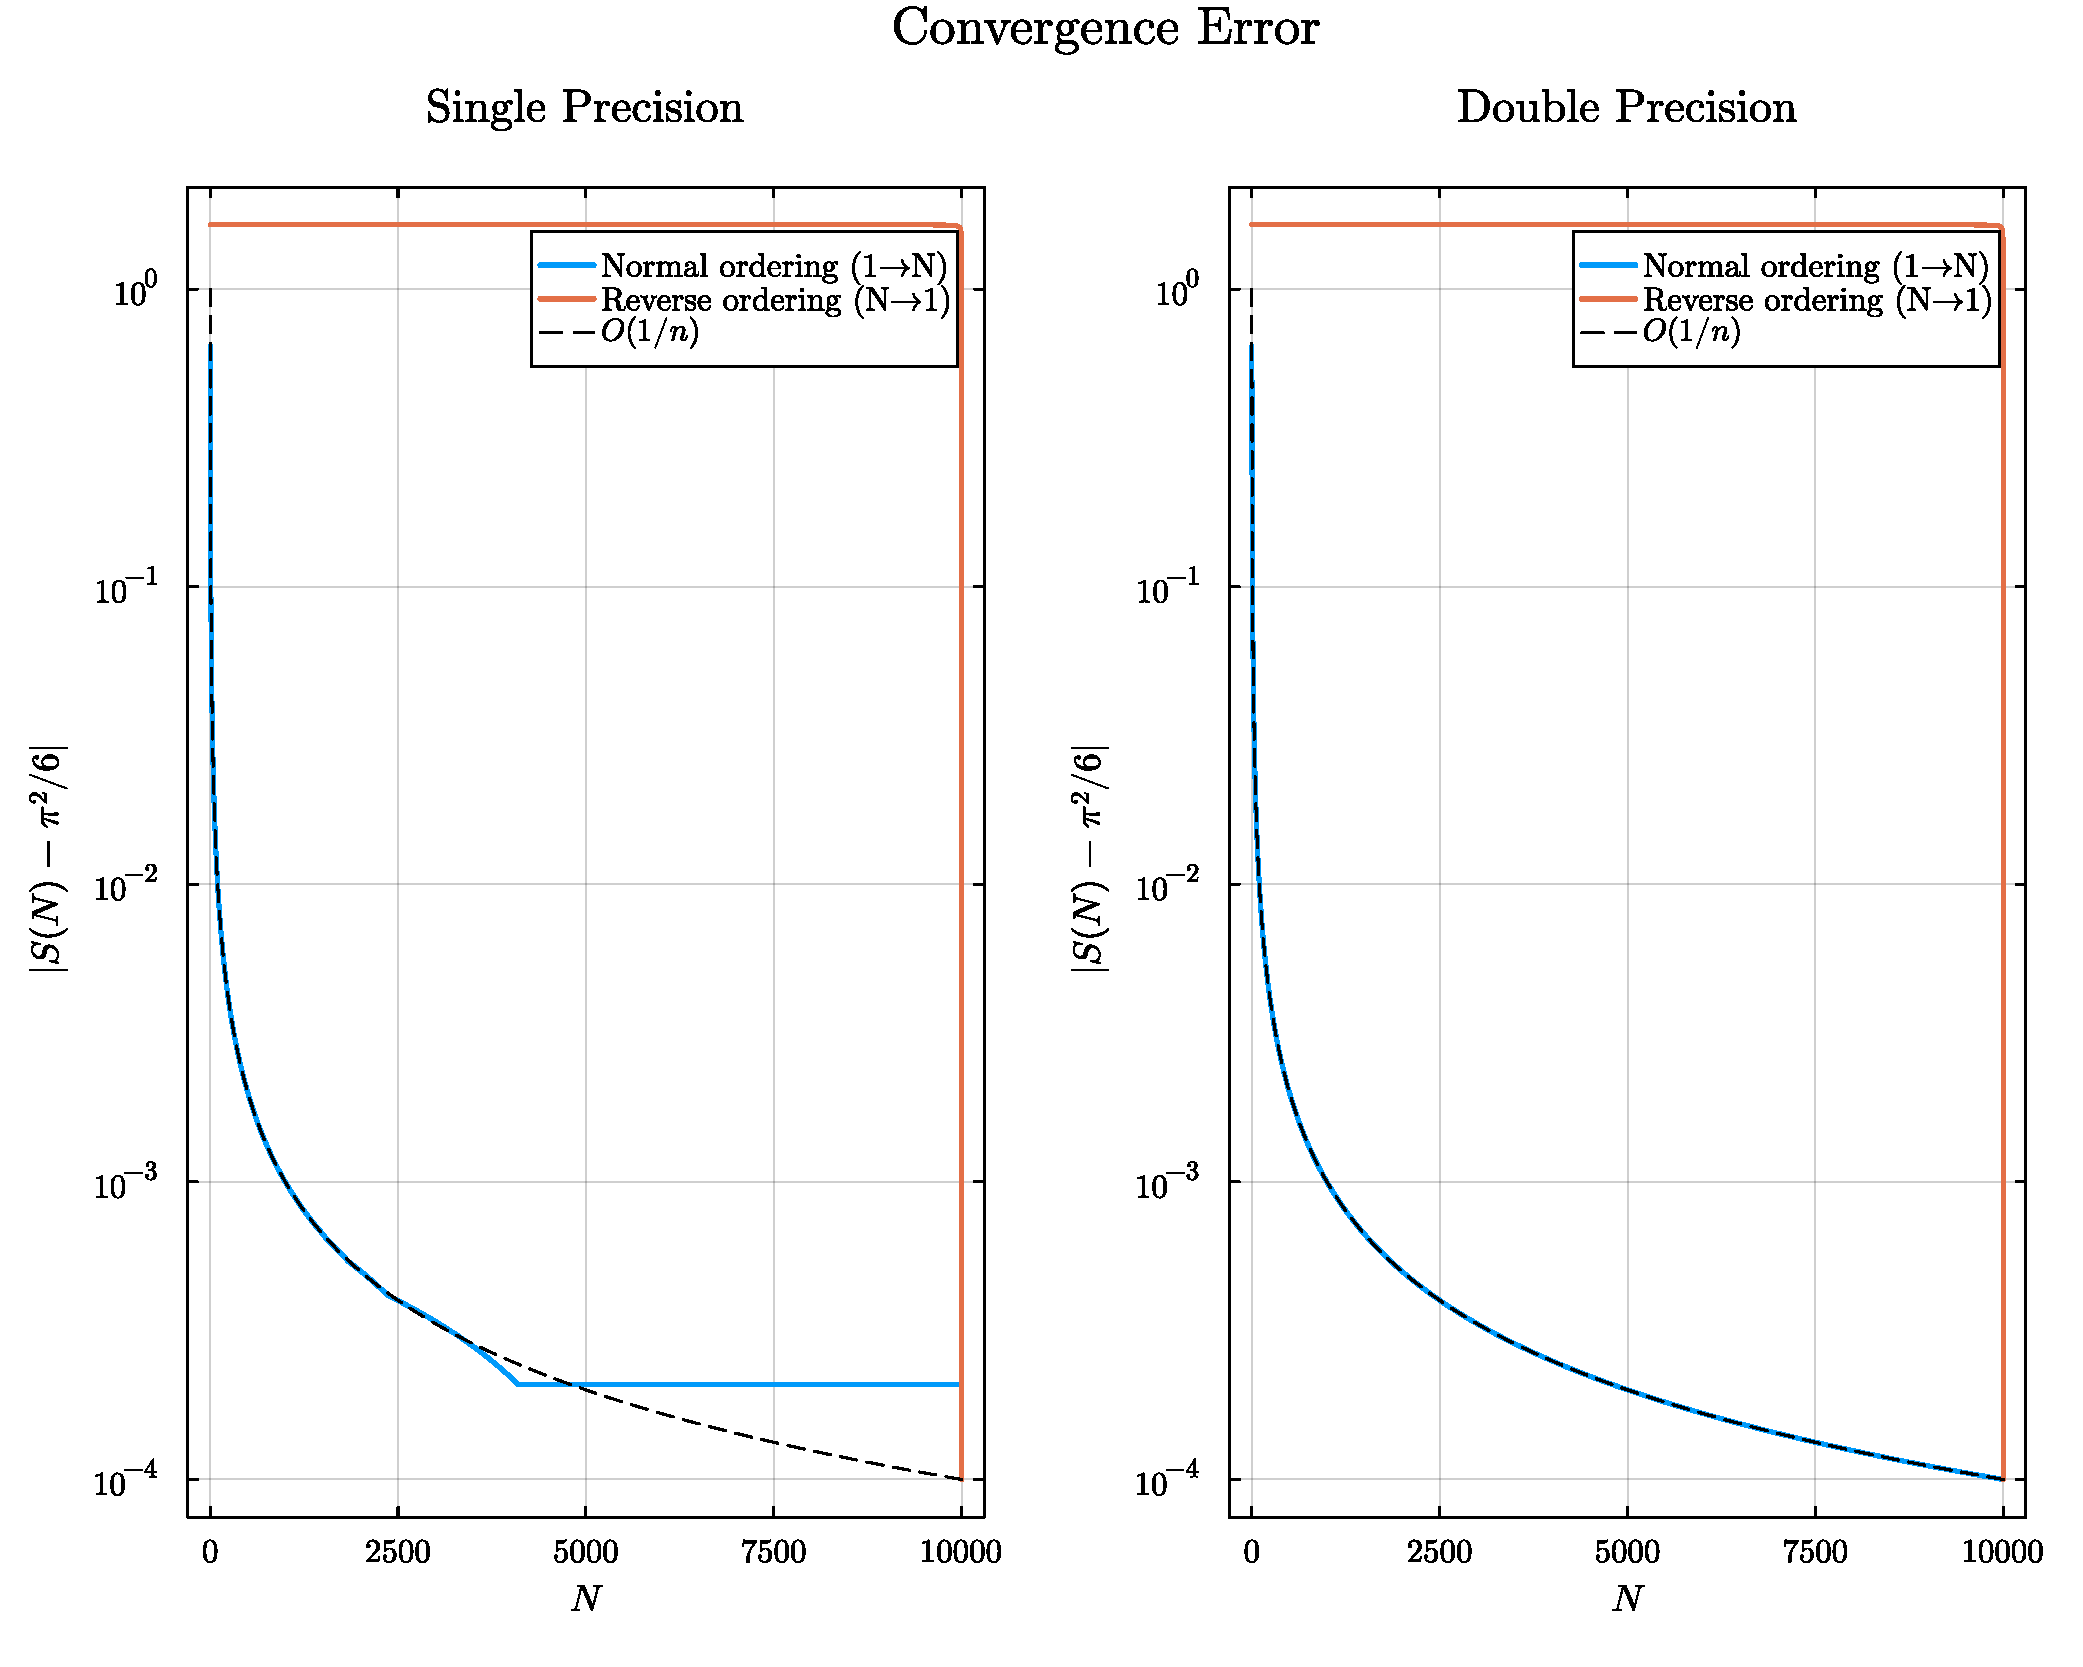
\includegraphics[width=0.8\textwidth]{figures/1-2/single_and_double_precision.pdf}
		\captionof{figure}{Log-log plot demonstrating the convergence of the normal
			and reverse sums in single and double precision against the $\mathcal{O}(1/N)$
			analytical truncation error.}
		\label{fig:convergence}
	\end{center}

	\paragraph{Discussion}
	The analytical sum converges to roughly $1.64493$. In \texttt{Float32}, the
	machine epsilon is $\epsilon_{32} \approx 1.19 \times 10^{-7}$. During normal
	ordering, the accumulator quickly grows to $\approx 1.64$. As $n$ increases, the
	added terms $1/n^2$ become exceedingly small. For example, at $n \approx 4000$,
	$1/n^2 \approx 6.25 \times 10^{-8}$. When adding this value to $1.64$, the
	magnitude difference exceeds the mantissa's bit-depth limit for single
	precision. The smaller numbers are effectively rounded off to zero, halting the
	accumulator's growth prematurely.

	Conversely, the reverse ordering fundamentally mitigates this issue. By
	summing the smallest numbers first, the accumulator remains comparable in
	magnitude to the terms being added. The accumulated tail eventually becomes
	large enough to effectively shift the mantissa of the lower-order integers
	(e.g., $n=1, 2$) when they are added at the very end of the loop.

	In double precision (\texttt{Float64}), the machine epsilon is vastly smaller
	($\epsilon_{64} \approx 2.22 \times 10^{-16}$). For $N = 10^6$, the smallest
	term is $1/10^{12} = 10^{-12}$, which is still well within the operational
	limits of double precision relative to an accumulator of $1.64$. Consequently,
	both the normal and reverse sums adhere smoothly to the theoretical analytical
	truncation error $\mathcal{O}(1/N)$ yielding equivalent errors of $\approx
		10^{-6}$.

	\paragraph{Conclusion}
	In finite-precision floating-point arithmetic (like \texttt{Float32}), the
	order in which you perform operations can significantly affect the result. This
	is especially true when adding numbers with very different sizes. If you add
	large numbers first, smaller ones can get “lost” due to rounding. By summing
	from the smallest values to the largest, you reduce these absorption errors and
	get a more numerically stable result.
\end{solution}

\subsection{Error Propagation and Condition Number}

\begin{exercise}
	\begin{enumerate}
		\item In statistics, we define the variance of a sample of values $x_1,\ldots,x_n$ by
		      \begin{equation}\label{eq:semplevar}
			      \sigma^2 = \frac{1}{n-1} \sum_{i=1}^n (x_{i} - \overline{x})^{2},
			      \qquad
			      \overline{x} = \frac{1}{n} \sum_{i=1}^n x_i.
		      \end{equation}
		      Write a function that takes as input a vector $x$ of any length and returns $\sigma^2$ as calculated by the formula. You should test your function with $x=[1,1,\ldots,1]$ and some random vectors.
		\item One drawback of the formula \eqref{eq:semplevar} is that you must first compute a sum for $\overline{x}$ before performing the sum to compute $\sigma^2$. This means that we have to pass twice through the data. This is undesirable for large data sets or when the sample variance is to be computed as the data is generated. Some textbooks quote a single-loop formula:
		      \[
			      \begin{split}
				      \sigma^2 = \frac{1}{n-1} \left( u - \tfrac{1}{n}v^2 \right), \\
				      u  = \sum_{i=1}^n x_i^2,
				      \qquad
				      v = \sum_{i=1}^n x_i.
			      \end{split}
		      \]
		      Try both formulas for the datasets below, each of which has a variance exactly equal to 1. Do this in both single and double precision.
		      \begin{align*}
			      x & = [ 1 \times 10^{3}, 1 + 1 \times 10^{3}, 2 + 1 \times 10^{3} ] \\
			      x & = [ 1 \times 10^{6}, 1 + 1 \times 10^{6}, 2 + 1 \times 10^{6} ] \\
			      x & = [ 1 \times 10^{7}, 1 + 1 \times 10^{7}, 2 + 1 \times 10^{7} ] \\
			      x & = [ 1 \times 10^{8}, 1 + 1 \times 10^{8}, 2 + 1 \times 10^{8} ] \\
		      \end{align*}
		      Can you explain the results?
	\end{enumerate}
\end{exercise}

\begin{solution}
	We implemented the two-pass algorithm in Julia using \texttt{sum()} and \texttt{broadcast} operations to ensure efficient computation. To investigate numerical stability, we compared this against the "single-pass" (or naive) algorithm. Both algorithms were evaluated using \texttt{Float32} and \texttt{Float64} types to observe the impact of machine epsilon ($\varepsilon_m$) on the final results.

	\paragraph{Results}
	Initial verification with a constant vector $x = [1, 1, 1, 1]$ yielded a variance of $0.0$ for both precisions, as expected. Random vector tests further confirmed the basic functionality of the \texttt{Float32} and \texttt{Float64} implementations. However, testing with shifted datasets revealed significant discrepancies, summarized in the table below:

	\begin{center}
		\centering
		\begin{tabular}{lcccc}
			\hline
			\textbf{Dataset Offset} & \textbf{Two-Pass (F32)} & \textbf{Two-Pass (F64)} & \textbf{One-Pass (F32)} & \textbf{One-Pass (F64)} \\ \hline
			$10^3$                  & 1.0                     & 1.0                     & 1.0                     & 1.0                     \\
			$10^6$                  & 1.0                     & 1.0                     & -131072.0               & 1.0                     \\
			$10^7$                  & 1.0                     & 1.0                     & 0.0                     & 1.0                     \\
			$10^8$                  & 0.0                     & 1.0                     & 0.0                     & 0.0                     \\ \hline
		\end{tabular}
		\captionof{table}{Comparison of variance calculations (True Variance = 1.0)}
	\end{center}

	\paragraph{Stability Analysis}
	As illustrated in Figure \ref{fig:stability_plot}, the relative error of the single-pass algorithm grows quadratically with the data offset. In \texttt{Float32}, the algorithm loses all precision once the offset exceeds $10^7$.

	\begin{center}
		\begin{center}
			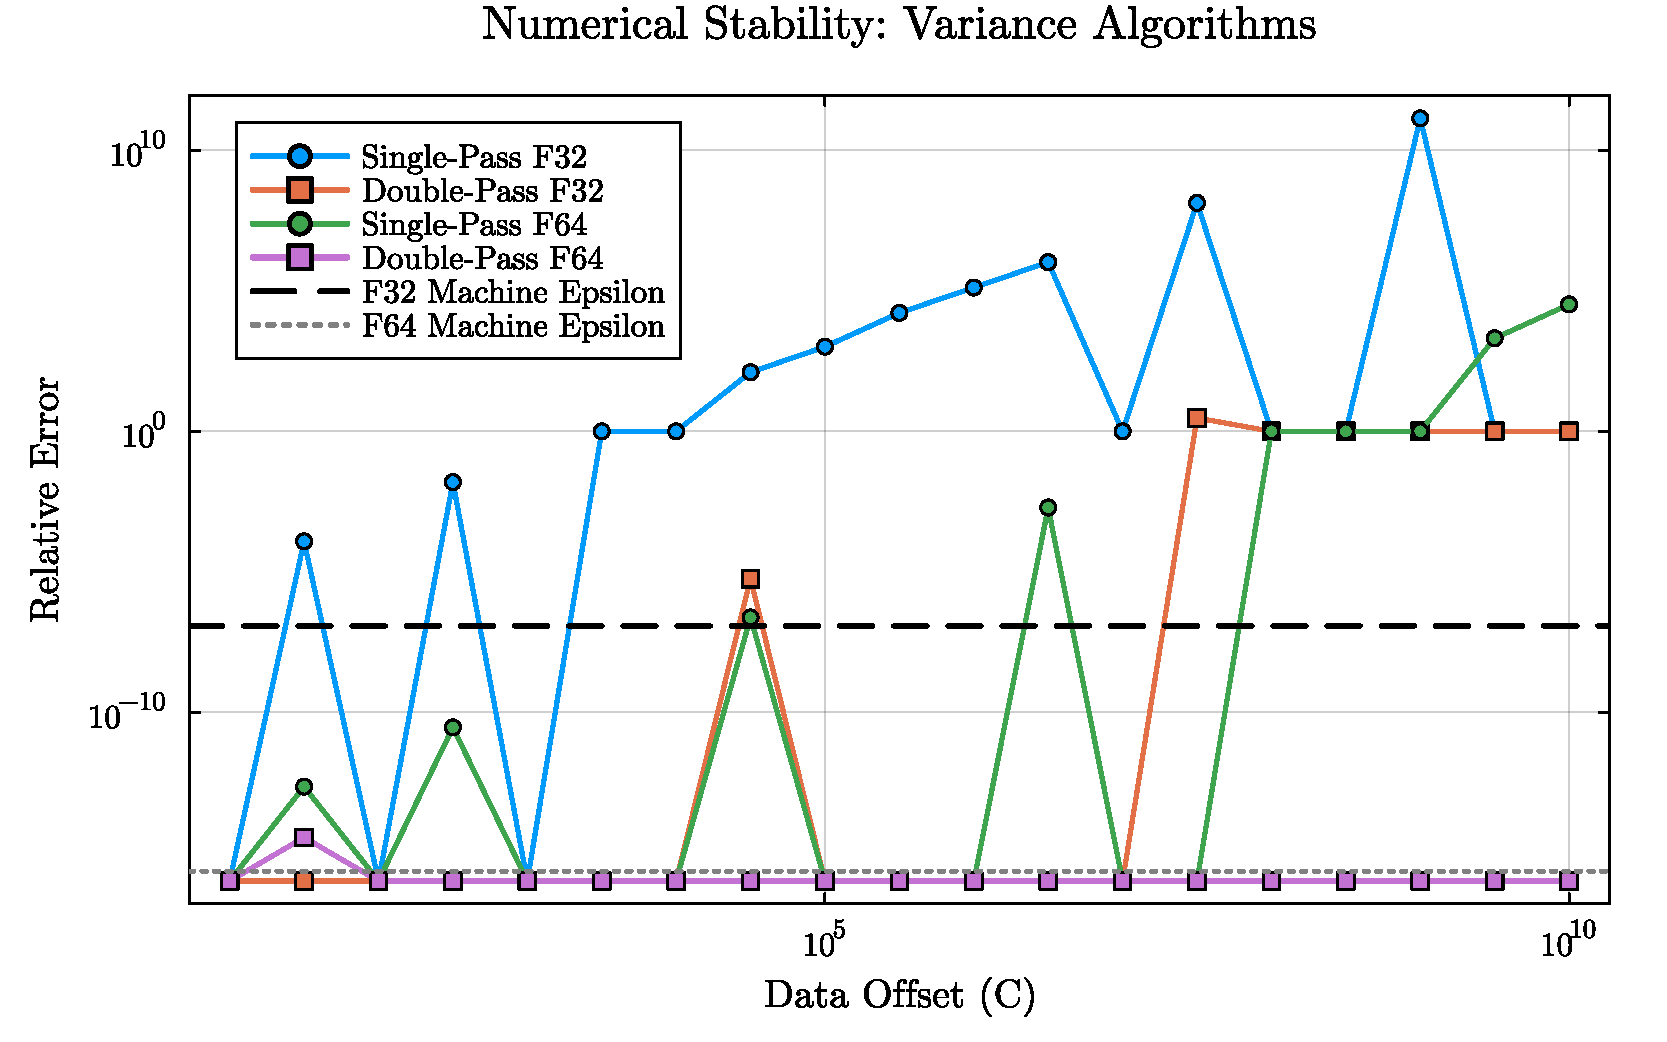
\includegraphics[width=0.95\textwidth]{figures/1-4/single_and_double_pass.pdf}
		\end{center}
		\captionof{figure}{Log-log plot comparing the relative error of single-pass and double-pass algorithms. Note the breakdown of the single-pass \texttt{Float32} implementation as the offset approaches the reciprocal of machine epsilon.}\label{fig:stability_plot}
	\end{center}


	\paragraph{Discussion}
	The failure of the single-pass algorithm is a classic example of \textbf{catastrophic cancellation}. The term $(u - \frac{1}{n}v^2)$ involves the subtraction of two very large, nearly identical numbers. When the offset (mean) of the data is large relative to the variance, the significant digits representing the variance are pushed beyond the precision limit of the floating-point representation.

	In \texttt{Float32}, which provides approximately 7 decimal digits of precision, the single-pass formula fails as early as $x \approx 10^6$. The result $-131072.0$ demonstrates that the cancellation error can lead to physically impossible (negative) variances. At $10^7$ and above, the result becomes $0.0$ because $u$ and $\frac{1}{n}v^2$ become identical in the representation. While \texttt{Float64} (approx. 15-17 digits) is more robust, it also succumbs to cancellation at $10^8$ for the single-pass method.

	\paragraph{Conclusion}
	The two-pass algorithm is significantly more \textbf{numerically stable} because it centers the data ($x_i - \overline{x}$) before squaring, thereby working with smaller magnitudes and preserving significant digits.
\end{solution}

\begin{exercise}
	Let \(f(x) = \frac{e^x-1}{x}\).
	\begin{enumerate}
		\item Find the condition number $\kappa_f(x)$. What is the maximum of $\kappa_f(x)$ over the interval \(-1\le x \le 1\)?
		\item Use the naive algorithm
		      \[
			      f(x)= \frac{e^{x}-1}{x}
		      \]
		      to compute \(f(x)\) at \(x=10^{-3},10^{-4},10^{-5},\ldots,10^{-16}\).
		\item Create a second algorithm from the first $n$ terms of the Maclaurin series, i.e.,
		      \[
			      p(x) = 1 + \frac{1}{2!}x + \frac{1}{3!}x^2 + \cdots + \frac{1}{(n+1)!}x^n.
		      \]
		      Evaluate it at the same values of $x$ as in part (2). To do this you have to choose a value for $n$. Check for the stability of the result when varying $n$. Could you have guessed a good value of $n$ from the start?
		\item Compare the results from the two implementations as a function of $x$. Which algorithm do you think is more accurate, and why?
	\end{enumerate}
\end{exercise}

\begin{solution}
	The evaluation of the function $f(x) = \frac{e^x - 1}{x}$ presents a classic challenge in numerical analysis due to \textit{catastrophic cancellation}. For small values of $x$, the term $e^x$ approaches unity, causing a loss of significant digits when performing the subtraction $e^x - 1$. To address this, we compare a direct "naive" implementation against a truncated Maclaurin series expansion. To establish a numerical "ground truth," we also utilize the built-in Julia function \texttt{expm1(x)}, which is specifically implemented to compute $e^x - 1$ with high precision for small arguments.

	The conditioning of the problem is analyzed via the relative condition number $\kappa_f(x)$:
	\[
		\kappa_f(x) = \left| \frac{x f'(x)}{f(x)} \right| = \left| \frac{x e^x}{e^x - 1} - 1 \right|
	\]

	\paragraph{Results}
	The condition number $\kappa_f(x)$ remains small throughout the domain $[-1, 1]$.
	\begin{itemize}
		\item \textbf{Maximum Condition Number:} $\kappa_f(1) = \frac{1}{e-1} \approx 0.58198$.
		\item \textbf{Behavior at the Origin:} $\lim_{x \to 0} \kappa_f(x) = 0$, confirming the problem is well-conditioned despite the removable singularity.
	\end{itemize}

	The naive algorithm was compared against the Maclaurin series for $x \in [10^{-16}, 10^{-3}]$. While the naive approach fails as $x \to \epsilon_{mach}$, the Maclaurin series remains stable.

	\begin{center}
		\centering
		\captionof{table}{Comparison of Naive vs. Maclaurin ($n=5$) algorithms for small $x$.}
		\begin{tabular}{cccc}
			\hline
			$x$        & \textbf{Naive} $f(x)$ & \textbf{Maclaurin} $p(x)$ & \textbf{Absolute Difference} \\
			\hline
			$10^{-3}$  & 1.00050016670838      & 1.00050016670834          & $4.28 \times 10^{-14}$       \\
			$10^{-8}$  & 0.99999999392253      & 1.00000000500000          & $1.11 \times 10^{-08}$       \\
			$10^{-12}$ & 1.00008890058234      & 1.00000000000050          & $8.89 \times 10^{-05}$       \\
			$10^{-15}$ & 1.11022302462516      & 1.00000000000000          & $1.10 \times 10^{-01}$       \\
			$10^{-16}$ & 0.00000000000000      & 1.00000000000000          & $1.00 \times 10^{+00}$       \\
			\hline
		\end{tabular}
	\end{center}

	% TODO: Increase the size of the image.
	\begin{center}
		\centering
		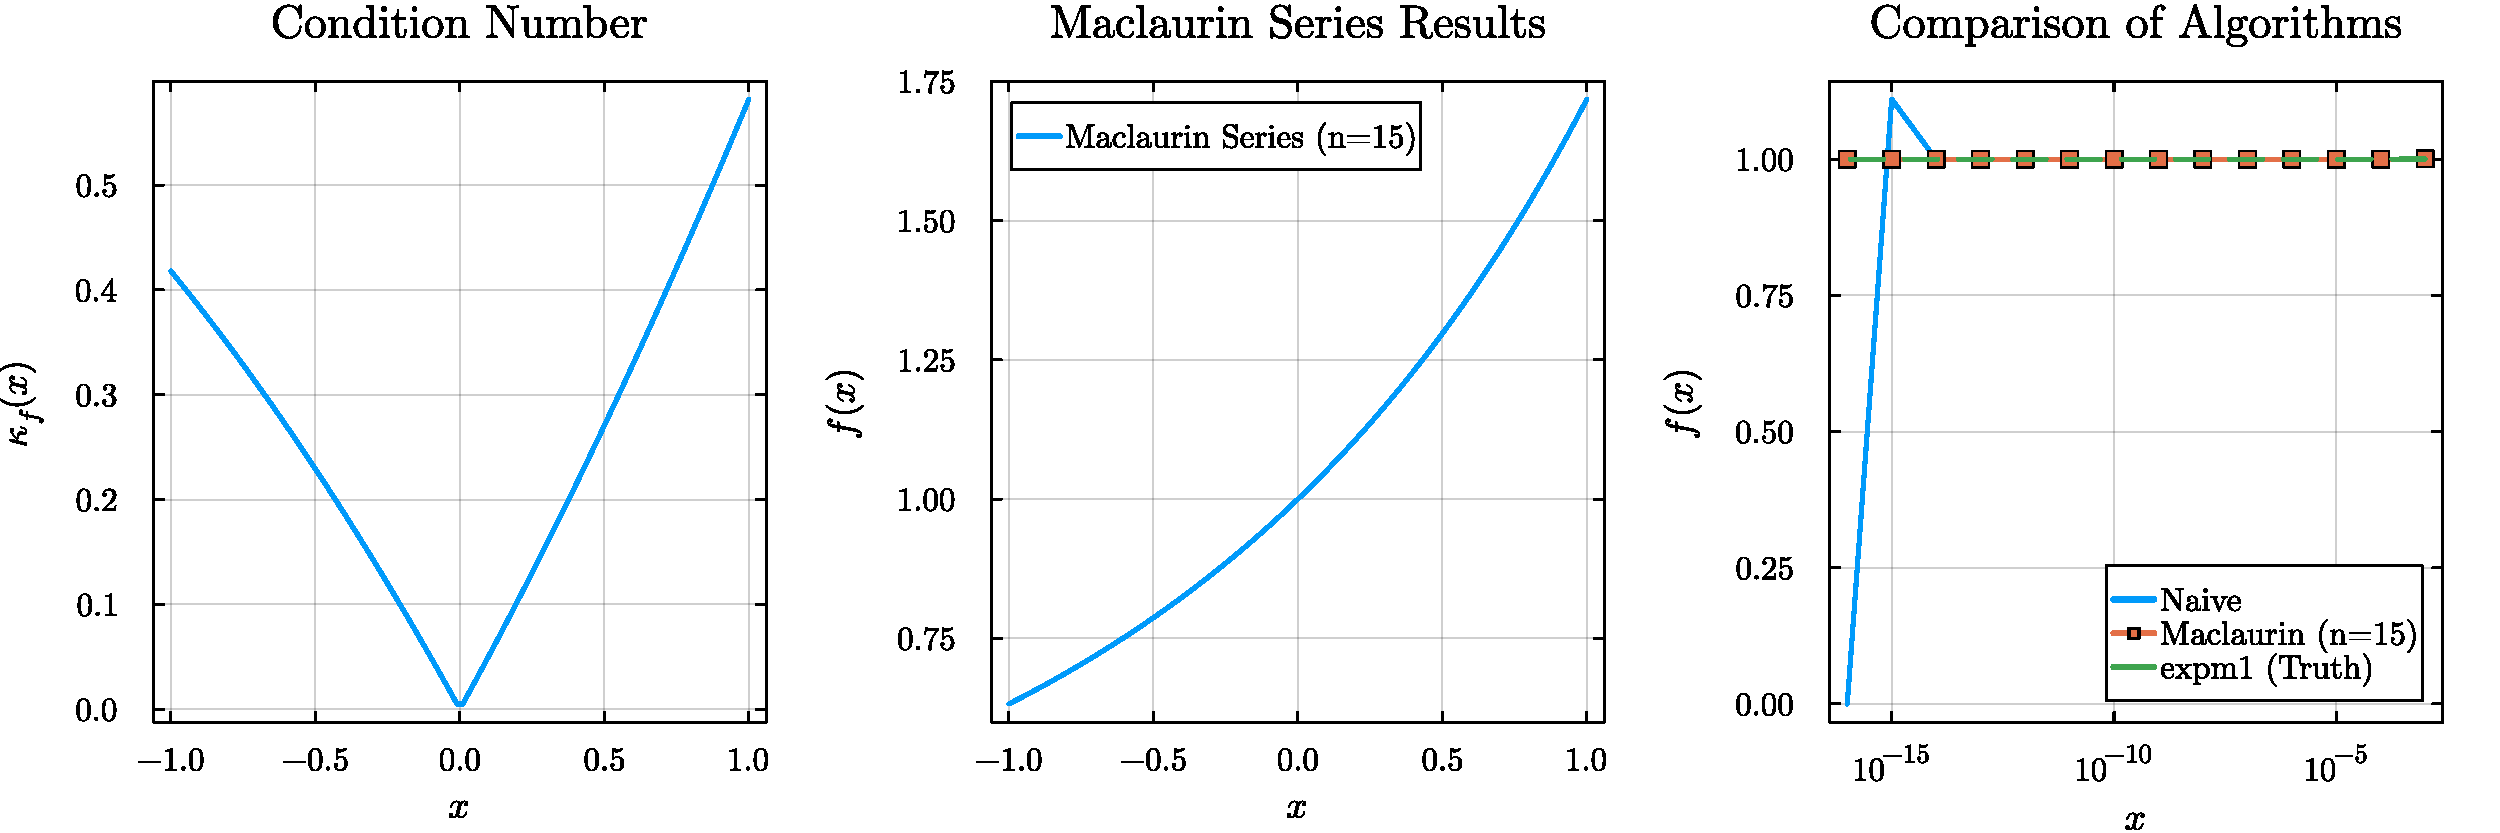
\includegraphics[width=0.9\textwidth]{figures/1-4/series_comparison.pdf}
		\captionof{figure}{Comparison of algorithms. The bottom panel demonstrates the catastrophic cancellation in the naive algorithm as $x \to 0$, while the Maclaurin approach tracks the stable \texttt{expm1(x)} baseline.}
		\label{fig:series_comparison}
	\end{center}

	\paragraph{Discussion}
	The instability of the naive algorithm is evident in Figure \ref{fig:series_comparison} for $x < 10^{-8}$. At $x=10^{-16}$, $e^x$ is rounded to $1.0$ in \texttt{Float64} precision, resulting in a computed value of $0$, a total loss of accuracy.

	In contrast, the Maclaurin series provides a robust alternative. To verify its accuracy, we compared the results against the Julia intrinsic \texttt{expm1(x)}. For $n=15$, the Maclaurin series and \texttt{expm1(x)} results are identical within machine precision, with an absolute difference of $0.0$ for nearly all tested values of $x$. This confirms that the Taylor expansion effectively reproduces the behavior of professional-grade numerical libraries in the vicinity of $x=0$.

	\paragraph{Conclusion}
	The Maclaurin series is significantly more accurate for small $|x|$ than the naive formula. The analysis demonstrates that even for well-conditioned problems ($\kappa_f \le 1$), algorithm choice is critical. For practical implementation, using optimized intrinsics like \texttt{expm1(x)} or switched logic (Taylor series for small $x$, naive for large $x$) is essential for numerical stability.
\end{solution}

% TODO: Add the comutational costs of all the algorighms used in this section.
